% Prof. Dr. Ausberto S. Castro Vera
% UENF - CCT - LCMAT - Curso de Ci\^{e}ncia da Computa\c{c}\~{a}o
% Campos, RJ,  2023
% Disciplina: Paradigmas de Linguagens de Programa\c{c}\~{a}o
%


\chapter{ Conceitos b\'{a}sicos da Linguagem R}

%Os livros b\'{a}sicos para o estudo da Linguagem R s\~{a}o: \cite{Cotton2013}, \cite{Kabacoff2015}, \cite{Wickham2016}, e \cite{Lander2017}, \cite{Chang2019}

%Um site sobre Cursos b\'{a}sicos R \'{e}:\\
 %\url{https://didatica.tech/curso-de-r-online-para-iniciantes/}

%Neste cap\'{\i}tulo \'{e} apresentado ....

%Segundo \cite{Sebesta2018}, a linguagem R,  . . .

%De acordo com \cite{Sebesta2018} e \cite{roy04}, a linguagem R . . .

\cite{Cotton2013} afirma que a linguagem R é, em seu cerne, imperativa, mas que também suporta programação orientada a objetos e programação funcional, ou seja, é uma linguagem multi-paradigmas. Sendo assim, essa "mistura" faz com que R tenha muitas similaridades com outras linguagens de programação. Podemos escrever códigos imperativos parecidos com os em C. Ou caso utilizemos as "Reference Class" vistas no capítulo passado, também somos capazes de construir algoritmos que se pareçam com os em Java. Buscando ser flexível nos métodos que utiliza para trabalhar com as principais áreas em que é inserida (Data science, Estatística, Big Data,etc.), R é utilizada por diversos tipos de desenvolvedores. Nesse capítulo aprenderemos a base dessa linguagem, o "esqueleto" que possibilita toda a movimentação diversificada do R. Aprenderemos como funcionam as suas variáveis, seus tipos de dados, suas operações e estruturas para começarmos a entender como se tornou uma linguagem tão abrangente.

%Considerando que a linguagem R (\cite{Sebesta2018}, \cite{wat90}) \'{e} considerada como ....

    %%%%%%%%=================================
    \section{Vari\'{a}veis e constantes}
    %%%%%%%%=================================
	Basicamente, uma variável é um espaço de armazenamento na memória do computador que pode conter um valor ou uma referência a um valor. Uma variável é identificada por um nome que é usado para acessar o seu valor ou referência. O valor contido nessa variável pode ser manipulado através de cálculos ou entradas do usuário.
	
	Já uma constante, é um valor que não pode ser alterado durante a execução do programa. Um valor fixo atribuído a uma variável no momento da sua declaração. 
	
	Vamos aprender como as variáveis e constantes são trabalhadas em R.Em R, as variáveis podem ser declaradas utilizando dois tipo de sintaxe de atribuição, sendo esses: "->" ou "=".
	Segue exemplo:
	
	\begin{figure}[H]
		\centering
		\caption{}
		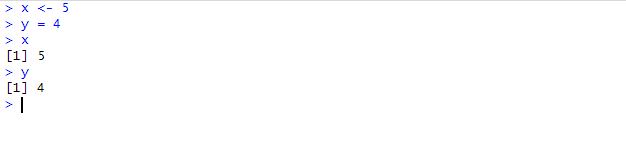
\includegraphics[width=1.0\linewidth]{Prints/screenshot001}
		\label{fig:screenshot001}
		{\tiny \sf Fonte: O autor deste trabalho }
	\end{figure} 
	
	
	Como dito acima, os valores atribuídos à variáveis podem ser manipulados através de cálculos ou entradas de usuários, segue exemplo abaixo de uma alteração do valor da mesma variável 'x' através de uma conta:
	\begin{figure}[H]
		\centering
		\caption{}
		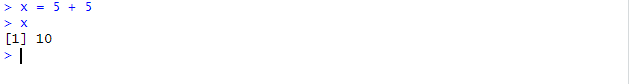
\includegraphics[width=1.0\linewidth]{Prints/screenshot002}
		\label{fig:screenshot002}
		{\tiny \sf Fonte: O autor deste trabalho }
	\end{figure} 
	
	Demonstramos, de uma forma básica, como declarar variáveis em R, atribuindo valores à elas. Utilizamos, nesse caso, o tipo de dado numeral, mas veremos no próximo tópico que em R existem diversos tipos de dados disponíveis.
	

    %%%%%%%%=================================
    \section{Tipos de Dados B\'{a}sicos}
    %%%%%%%%=================================
    
    A linguagem R tem uma variedade de tipos de dados, vamos lista-los e fazer uma breve descrição de cada um. São esses:
    \subsection{Dados numéricos}
    	Demonstrados nos exemplos acima, os dados numéricos em R são utilizados para armazenar valores como inteiros, reais e complexos.Existem dois tipos principais de números: inteiros e de ponto flutuante. Os números inteiros são números sem frações, enquanto os números de ponto flutuante têm uma parte fracionária. O R também suporta números que possuam uma parte real e imaginária.\par
    	Porém, esse tipo de dado, possui algumas limitações, como por exemplo, como visto em \cite{Cotton2013}, limitação na precisão, esse tipo de dado pode sofrer com cálculos que possuem números grandes demais ou pequenos demais. Outro exemplo de limitação seria o arredondamento, algumas operações matemáticas podem gerar resultados arredondados, o que pode levar a erros em cálculos que dependem de alta precisão.
    \subsection{Dado de caracteres}
    	Outro tipo de dado existente em R é o de texto, ou caracteres, é utilizado para armazenar texto, palavras e frases, além de códigos alfanuméricos. Uma string (basicamente, uma sequência de caracteres que podem ser letras, números, símbolos ou até espaços em branco) é criada ao colocar o texto entre aspas simples('') ou duplas ("").\par
    	As strings em R são tratadas como vetores de caracteres, permitindo operações como a seleção de um ou mais caracteres específicos, a seleção de subconjuntos de caracteres e a combinação de diferentes strings.\par 
    	Entretanto, esse tipo de dado também possui algumas limitações, como por exemplo, o tamanho máximo de uma string, apesar de poder variar com a versão do R e do sistema operacional utilizado, ainda pode ser um problema em casos de manipulação de textos muito longos, como em análises de textos de grande extensão. Além dessa, pode ser citado o tratamento de caracteres especiais, algumas linguagens, incluindo o R, podem ter dificuldades em manipular caracteres como acentos e outros símbolos, podendo afetar a utilização e processamento de textos em línguas que utilizam esses caracteres.
    \subsection{Dados lógicos}
    	Os dados lógicos, também conhecidos como booleanos, possibilitam a representação de valores verdadeiros ou falsos. Em R, o valor verdadeiro é representado pela palavra chave 'TRUE' e o valor falso, pela palavra chave 'FALSE'.\par 
    	Esses valores lógicos são frequentemente utilizados em operações de condição e controle de fluxo, como nos comandos 'if', 'else', 'while' e 'for'. Essas operações podem funcionar se baseando no valor lógico dessas variáveis.\par 
    	Apesar de simples, os valores lógicos são fundamentais na programação para controlar o fluxo da execução do programa.\par 
    	Todavia, também possui limitações, sendo elas o fato de os valores lógicos serem limitados a dois estados (verdadeiro ou falso), o que significa que eles não podem representar nuances ou escalas de valores. Além disso, operações lógicas podem ser um pouco mais complexas e difíceis de entender, especialmente quando há várias condições envolvidas.
    	
    	

     %%%%%%%%=================================
    \section{Tipos de Dados de Cole\c{c}\~{a}o}
    %%%%%%%%=================================
    	De acordo com \cite{Laureano2008}, os tipos de dados podem ser divididos dois grupos: atômicos e complexos, atômicos sendo o que nós estudamos acima, aqueles cujos elementos do conjunto de valores são indivisíveis, como são os inteiros, caracteres e lógicos. Agora estudaremos os complexos (ou compostos, ou de coleção) que, por sua vez, são aqueles cujos elementos do conjunto de valores podem ser decompostos em partes mais simples. Entenderemos melhor a partir de uma explicação mais detalhada de cada um existente em R.
    	
    \subsection{Vetores}
    		Os vetores são as coleções mais simples do R, e podem ser criados com diferentes classes de dados, como numéricos, inteiros, caracteres, fatores e lógicos. Eles podem ser considerados como uma sequência unidimensional de elementos de um mesmo tipo, e podem ser acessados e manipulados por meio de índices. São úteis em casos como se você deseja armazenar os dados totais de 50 clientes, em vez de criar 50 variáveis diferentes para cada um, basta criar um vetor de comprimento 50, que vai armazenar assim todos os dados do clientes.Vetores são estruturas de dados que podem ser declaradas com a função 'c()'. Como no exemplo abaixo:\begin{figure}[H]
    			\centering
    			\caption{}
    			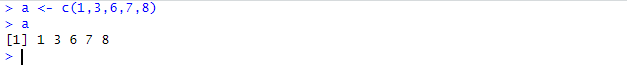
\includegraphics[width=1.0\linewidth]{Prints/screenshot003}
    			\label{fig:screenshot003}
    			{\tiny \sf Fonte: O autor deste trabalho }
    		\end{figure}
    		
    		Como limitação, existe o fato de que os vetores não funcionam com tipos diferentes de dados. Um vetor não pode ter números e caracteres dentro dele, por exemplo.
    \subsection{Listas}
    		As listas, por sua vez, são coleções que podem armazenar elementos de diferentes tipos e dimensões. Cada elemento da lista pode ser um vetor, uma matriz, uma outra lista, ou até mesmo um objeto R qualquer. As listas podem ser manipuladas de diversas formas, como adicionar ou remover elementos, modificar elementos existentes, ou até mesmo acessar elementos específicos utilizando índices.\par 
    		As listas podem ser declaradas com a função 'list()'. Abaixo um exemplo de uma lista sendo criada com três tipos diferentes de dados (uma lista, um vetor e um numeral.):\begin{figure}[H]
    			\centering
    			\caption{}
    			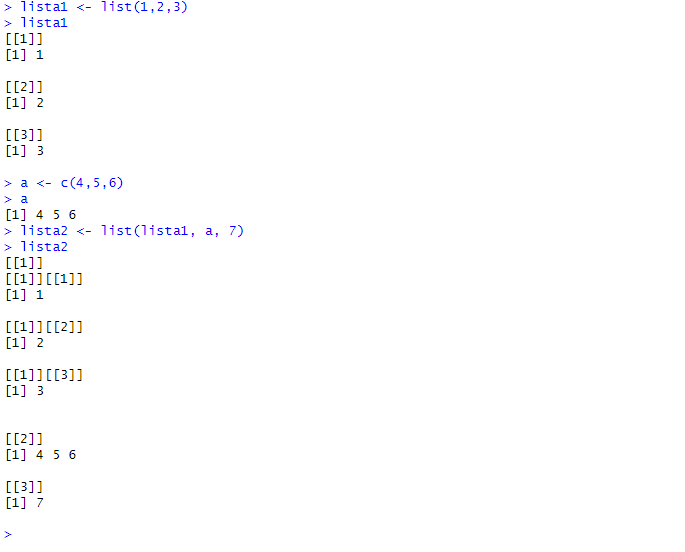
\includegraphics[width=1.0\linewidth]{Prints/screenshot004}
    			\label{fig:screenshot004}
    			{\tiny \sf Fonte: O autor deste trabalho }
    		\end{figure}
    		Embora as listas sejam flexíveis e úteis para muitas aplicações, é importante levar em consideração algumas limitações, como por exemplo, a manipulação de uma lista pode ter seu índice um pouco confuso, já que seus elementos podem ser de diferentes tipos e tamanhos.
    \subsection{Matrizes}
    		 Assim como os vetores, as matrizes são coleções de elementos do mesmo tipo, entretanto, são bidimensionais e organizadas em linhas e colunas. Podem ser criadas a partir de vetores, ou diretamente utilizando a função 'matrix()'. A sintaxe da função é, basicamente, 'matrix(dados, nrow = r, ncol = c, byrow = FALSE)' dentro dela, podemos definir o número de linhas (nrow), colunas (ncol) e se os dados serão inseridos por colunas (byrow = FALSE) ou linhas (byrow = TRUE). Segue exemplo:\begin{figure}[H]
    		 	\centering
    		 	\caption{}
    		 	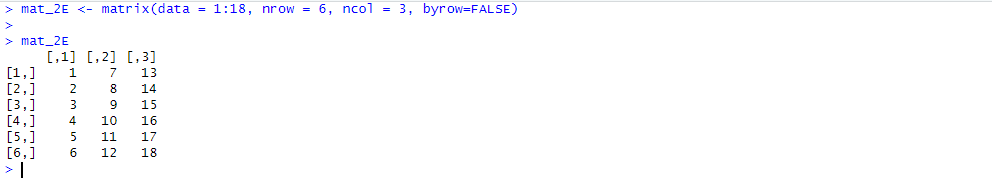
\includegraphics[width=1.5\linewidth]{Prints/screenshot005}
    		 	\label{fig:screenshot005}
    		 	{\tiny \sf Fonte: O autor deste trabalho }
    		 \end{figure}
    	 	 Compartilhando da limitação dos vetores, as matrizes não podem receber mais de um tipo de dados em sua estrutura, além de serem fixas em tamanho, ou seja,o número de linhas e colunas deve ser especificado no momento da criação da matriz. Se você precisar adicionar ou remover linhas ou colunas, pode ser necessário criar uma nova matriz ou transformá-la em outro tipo de estrutura de dados.
    \subsection{DataFrame}
    		Por fim, temos os dataframes, sendo uma forma mais generalizada das matrizes, contém dados de forma tabular e cada coluna de sua estrutura pode conter tipos diferentes de dados. Em resumo, enquanto as matrizes em R são estruturas de dados bidimensionais com elementos do mesmo tipo, os data frames são mais flexíveis e permitem diferentes tipos de dados em cada coluna. Por isso, os data frames são frequentemente usados em análise de dados e modelagem estatística em R. Além da fácil visualização, manipulação e analise por conta de seu modelo tabular. Exemplo:\begin{figure}[H]
    			\centering
    			\caption{}
    			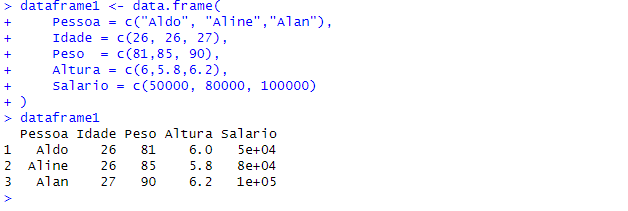
\includegraphics[width=1.0\linewidth]{Prints/screenshot006}
    			\label{fig:screenshot006}
    			{\tiny \sf Fonte: O autor deste trabalho }
    		\end{figure}
    		Apesar de amplamente utilizado por conta de sua flexibilidade e utilidade, o dataframe possui limitações, como o fato de não serem adequados para representar dados com mais de duas dimensões ou por ter a necessidade de que todos os elementos de um dataframe tenham o mesmo comprimento.

     %%%%%%%%=================================
    \section{Opera\c{c}\~{o}es L\'{o}gicas}
    %%%%%%%%==================================
    Operações lógicas são operações matemáticas que retornam valores lógicos, isto é, verdadeiro (TRUE) ou falso (FALSE). Em R, essas operações podem ser listadas em:\begin{itemize}
    	\item Operador de igualdade: '=='
    	\item Operador de desigualdade: '!='
    	\item Operador de maior que: '>'
    	\item Operador de menor que: '<'
    	\item Operador de maior ou igual que: '>='
    	\item Operador de menor ou igual que: '<='
    	\item Operador lógico AND: '\&' ou '\&\&'
    	\item Operador lógico OR: '|' ou '||'
    	\item Operador lógico NOT: '!'
    \end{itemize}
	Esses operadores retornam valores lógicos (TRUE ou FALSE) com base nas condições que são avaliadas. Por exemplo, se você quiser verificar se um número x é maior que 5, você pode usar o operador de maior que (>):\begin{figure}[H]
		\centering
		\caption{}
		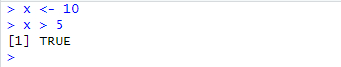
\includegraphics[width=0.7\linewidth]{Prints/screenshot007}
		\label{fig:screenshot007}
		{\tiny \sf Fonte: O autor deste trabalho }
	\end{figure}
	Operações lógicas podem também possuir mais de um operador, por exemplo, é possível usar operadores lógicos para combinar múltiplas condições. Por exemplo, se você quiser verificar se um número x está entre 5 e 10, você pode usar o operador lógico AND (\&):\begin{figure}[H]
		\centering
		\caption{}
		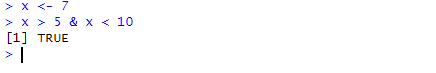
\includegraphics[width=0.7\linewidth]{Prints/screenshot008}
		\label{fig:screenshot008}
		{\tiny \sf Fonte: O autor deste trabalho }
	\end{figure}
	


    %%%%%%%%=================================
    \section{Estrutura de Controle e Fun\c{c}\~{o}es}
    %%%%%%%%=================================
  	De acordo com \cite{Kabacoff2015}, as declarações de um programa em R são executadas sequencialmente do topo do código até o fim. Porém, em alguns casos, é necessário que alguma dessas declarações seja executada repetidas vezes, enquanto em outros casos, que só seja executada caso cumpra algumas condições. e é onde entram as estruturas de controle.\par 
  	Essas estruturas podem ser dividas em dois tipos: iterativas e condicionais. Veremos das duas:
  	\subsection{Iterativas}
  		As estruturas iterativas, como o nome sugere, são usadas para iterar sobre um conjunto de dados. As principais estruturas iteradoras em R são: "for" e "while".
  		\subsubsection{For}
  			A estrutura 'for' executa uma declaração repetidamente até que o valor de uma variável de controle alcance um valor ja estabelecido nos parâmetros da função. Sua sintaxe é 'for (var in seq)' var sendo a variável de controle e seq o valor final que ela alcança. Nesse exemplo:\begin{figure}[H]
  				\centering
  				\caption{}
  				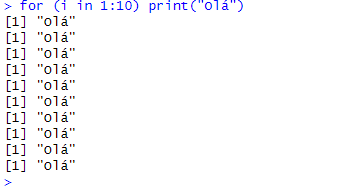
\includegraphics[width=0.7\linewidth]{Prints/screenshot009}
  				\label{fig:screenshot009}
  				{\tiny \sf Fonte: O autor deste trabalho }
  			\end{figure}
  			'Olá' foi imprimido 10 vezes.
  		\subsubsection{While}
  			A estrutura 'while' executa uma declaração repetidamente enquanto a condição dentro da estrutura for verdadeira. A sintaxe é 'while (cond) declaração'. Nesse exemplo:\begin{figure}[H]
  				\centering
  				\caption{}
  				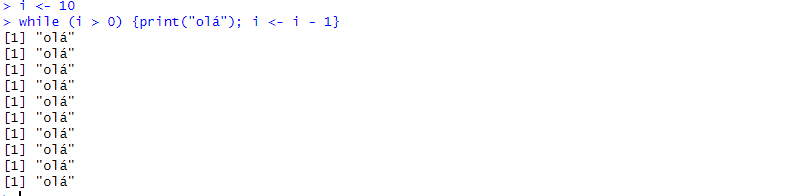
\includegraphics[width=1.0\linewidth]{Prints/screenshot010}
  				\label{fig:screenshot010}
  				{\tiny \sf Fonte: O autor deste trabalho }
  			\end{figure}
  			'Olá' foi novamente imprimido 10 vezes. Nessa estrutura é importante observar que é necessário uma modificação da variável de controle, dentro do bloco da declaração, que faça a condição ser alcançada, caso contrário, o while entrará em um loop infinito.
  	\subsection{Condicionais}
  		Nas estruturas condicionais, uma declaração só sera executada se uma condição especificada for alcançada. Essas são a 'if-else' e 'switch'.
  		\subsubsection{If-else}
  			A estrutura if-else executa uma declaração se uma condição específica for verdadeira. Opcionalmente, uma outra declaração pode ser executada, caso a condição seja falsa. A sintaxe é 'if (cond) declaração' ou 'if (cond) declaração1 else declaração2'. Nesse exemplo:\begin{figure}[H]
  				\centering
  				\caption{}
  				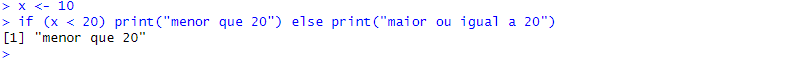
\includegraphics[width=1.0\linewidth]{Prints/screenshot011}
  				\label{fig:screenshot011}
  				{\tiny \sf Fonte: O autor deste trabalho }
  			\end{figure}
  			A primeira declaração foi executada, visto que a condição retornou verdadeira (x era menor que 20).

		\subsubsection{Switch}
			A estrutura switch em R é usada para realizar a seleção entre várias alternativas com base em uma expressão de teste. O switch é frequentemente usado em R para substituir uma longa sequência de if-else quando se trata de testar uma única variável em várias condições. A sintaxe é 'switch(expressão, caso1, caso2, caso2, ..., casoN)'. No exemplo abaixo:\begin{figure}[H]
				\centering
				\caption{}
				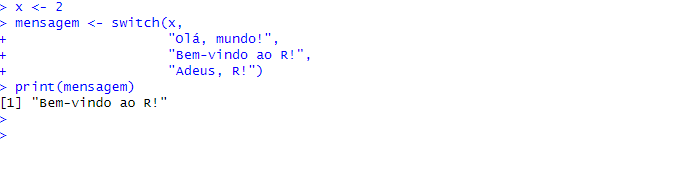
\includegraphics[width=1.0\linewidth]{Prints/screenshot012}
				\label{fig:screenshot012}
				{\tiny \sf Fonte: O autor deste trabalho }
			\end{figure}
			a variável 'mensagem' recebeu e imprimiu a segunda frase, pois x = 2.\par 
	
	Por fim, além das estruturas de controle, R possui como grande vantagem o fato do usuário ser capaz de adicionar funções. As funções em R são blocos de código que executam uma tarefa específica e retornam um valor. Elas permitem que você reutilize o mesmo código várias vezes em seu programa, tornando o seu código mais modular e mais fácil de manter e modificar. A estrutura de uma função é essa 'minhaFuncao <- function(arg1, arg2, ...){declaracoes return(object)}' seguido da declaração 'function' estão os argumentos da função entre os parênteses e o corpo da função entre as chaves. Um exemplo simples:\begin{figure}[H]
		\centering
		\caption{}
		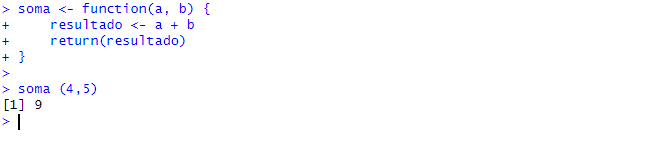
\includegraphics[width=1.0\linewidth]{Prints/screenshot013}
		\label{fig:screenshot013}
		{\tiny \sf Fonte: O autor deste trabalho }
	\end{figure}
	Nesse exemplo, os números passados como argumentos são o 4 e o 5, foram somados dentro da função e o resultado foi retornado. Apesar da função do exemplo ter sido simples, as funções podem ter todos os tipos de estruturas estudados (inclusive outras funções ou até mesmo a própria função executada), é um bloco de código que pode ser chamado a qualquer momento com diversos tipos de argumentos.

    %%%%%%%%======================
    \section{M\'{o}dulos}
    %%%%%%%%======================
	Como dito acima, uma função pode ter em si todos os tipos de estruturas, o que facilita a modulação e a manutenção do programa, dessa forma, possibilitando a criação de módulos na linguagem R. Módulos podem ser definidos como conjuntos de funções e objetos relacionados.Um módulo é um conjunto de funcionalidades que podem ser agrupadas e organizadas em um pacote para facilitar a reutilização e a manutenção do código. Assim como as funções facilitam a manipulação do código em um ponto de vista mais fechado, os módulos fazem de uma forma mais ampla com o programa, o modularizando e permitindo a reutilização, caso necessário. Além disso, cada módulo pode ter sua própria documentação, permitindo que os usuários entendam facilmente como as funções e objetos do módulo são usados e quais são suas finalidades específicas.\par 
	Como visto no primeiro capítulo, um dos destaques da linguagem R é a sua ampla oferta de pacotes que fornecem módulos para tarefas específicas.Pode se dizer então que os pacotes estão para os módulos, como os módulos estão para as funções, do ponto de vista da modularização do programa. Em resumo, as funções são a menor unidade de funcionalidade, os módulos são um conjunto de funções e objetos relacionados e os pacotes são um conjunto de módulos, dados e documentação relacionados. A modularização do código em R é uma prática recomendada para garantir a reutilização e a manutenção do código.\par 
	Para finalizar, um exemplo de pacote poderia ser o "ggplot2" que, por sua vez, contém vários módulos, como o "scale", "theme e "geom", cada um com funções e objetos específicos para diferentes aspectos da criação de gráficos.


    %%%%%%%%======================
    \section{Orienta\c{c}\~{a}o a Objetos}
    %%%%%%%%======================
	A orientação a objetos é uma abordagem de programação que enfatiza a criação de objetos que têm atributos (variáveis) e métodos (funções) que podem ser acessados e manipulados por outros objetos ou funções.
	Como visto no começo desse capítulo, R não é uma linguagem puramente orientada a objetos, mas tem características desse paradigma, em \cite{Cotton2013}, aprendemos que, em R, todas as funções, em si, são objetos de primeira classe, e de fato, de acordo com o próprio criador da linguagem R, John Chambers, "Tudo o que existe em R é um objeto". Em algumas circunstâncias, é útil aproveitar do estilo de POO presente em R, e pra isso é necessário entender como funcionam os três diferentes sistemas de Orientação a Objetos existentes em R.
	\subsection{S3}
		Em R, a classe S3 não possui uma definição pré-definida e não segue uma estrutura rígida de programação orientada a objetos como em outras linguagens como Java, C++ e C\#. Em vez disso, a implementação de S3 é baseada na passagem de mensagens genéricas para métodos específicos, o que torna a implementação mais flexível e fácil de usar. Dessa forma, a função genérica age como um intermediário que despacha a chamada para o método específico correspondente à classe do objeto em questão.\par 
		Para criar um objeto S3, basta atribuir a ele uma classe definida pelo usuário usando a função class(). Por exemplo:\begin{figure}[H]
			\centering
			\caption{}
			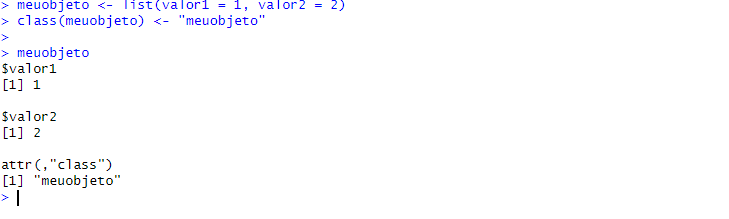
\includegraphics[width=1.0\linewidth]{Prints/screenshot014}
			\label{fig:screenshot014}
			{\tiny \sf Fonte: O autor deste trabalho }
		\end{figure}
	\subsection{S4}
		O S4 é um sistema de orientação a objetos mais formalizado em R do que o S3, com definições mais precisas e estritas para classes e métodos. Diferente do S3, as classes S4 são definidas explicitamente, com o uso da função setClass(), que define os slots (atributos) e métodos associados a uma determinada classe. Além disso, para adicionar um método a uma classe S4 em R, é preciso usar a função setGeneric() para criar uma função genérica (como uma interface) que irá definir o nome e a assinatura da função. Em seguida, é necessário usar a função setMethod() para criar a implementação dessa função genérica para a classe específica. \par 
		Um exemplo de um objeto em S4 em R seria a definição de uma classe "Pessoa", com atributos como "nome" e "idade", e métodos como "aniversario" para incrementar a idade da pessoa em 1 ano:\begin{figure}[H]
			\centering
			\caption{}
			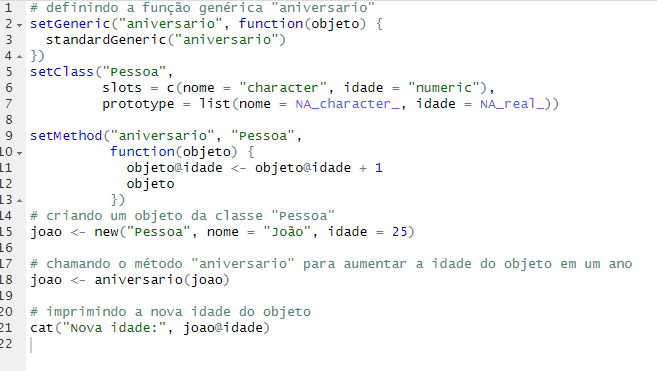
\includegraphics[width=1.0\linewidth]{Prints/screenshot015}
			\label{fig:screenshot015}
			{\tiny \sf Fonte: O autor deste trabalho }
		\end{figure}
		O resultado da última linha será "Nova idade: 26".
	\subsection{Reference Class}
		Reference Class já é um sistema de orientação a objetos mais próximos dos robustos das linguagens realmente voltadas a esse paradigma.No RC, os objetos são criados como instâncias de uma classe específica, e essa classe pode ter propriedades (ou atributos) e métodos, que podem ser acessados e modificados de forma semelhante à essas linguagens. Basicamente, tem todas as propriedades do S4, mas com mais estruturas e restrições. Exemplo:\begin{figure}[H]
			\centering
			\caption{}
			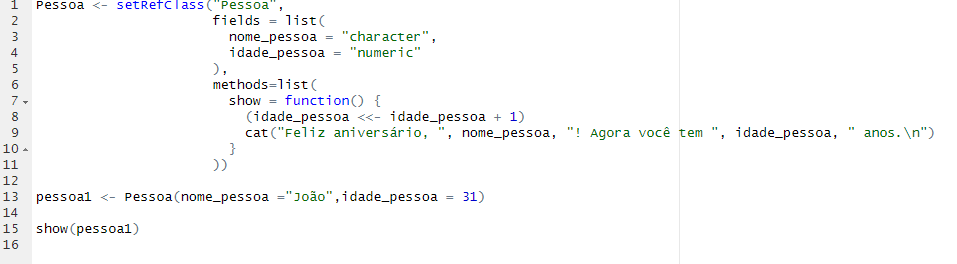
\includegraphics[width=1.0\linewidth]{Prints/screenshot016}
			\label{fig:screenshot016}
			{\tiny \sf Fonte: O autor deste trabalho }
		\end{figure}
		O resultado da última linha sendo: "Feliz aniversário,  João ! Agora você tem  32  anos."
		
